\documentclass[12pt,a4paper]{article}
\usepackage[utf8]{vietnam}
\usepackage[utf8]{inputenc}
\usepackage{tabto}
\usepackage{amsmath}
\usepackage{amsfonts}
\usepackage{multicol}
\usepackage{tikz}
\usepackage{amssymb}
\usepackage{listings}
\usepackage[left=2cm,right=2cm,top=2cm,bottom=2cm]{geometry}
\usepackage{graphicx}
\usepackage{xcolor}
\usepackage{wrapfig}
\usepackage[font=small,labelfont=bf]{caption}
\usepackage{hyperref}
\usepackage{tikz}
\usetikzlibrary{datavisualization}
\usetikzlibrary{datavisualization.formats.functions}
\graphicspath{ {./images/} }
\author{Trần Đức Mạnh}
\title{Course 1: Linear Algebra for Machine Learning \& Data Science\\Overview}

\definecolor{codegreen}{rgb}{0,0.6,0}
\definecolor{codegray}{rgb}{0.5,0.5,0.5}
\definecolor{codepurple}{rgb}{0.58,0,0.82}
\definecolor{backcolour}{rgb}{0.95,0.95,0.92}

\lstdefinestyle{mystyle}{
    backgroundcolor=\color{backcolour},   
    commentstyle=\color{codegreen},
    keywordstyle=\color{magenta},
    numberstyle=\tiny\color{codegray},
    stringstyle=\color{codepurple},
    basicstyle=\ttfamily\footnotesize,
    breakatwhitespace=false,         
    breaklines=true,                 
    captionpos=b,                    
    keepspaces=true,                 
    numbers=left,                    
    numbersep=5pt,                  
    showspaces=false,                
    showstringspaces=false,
    showtabs=false,                  
    tabsize=2
}

\lstset{style=mystyle}

\begin{document}
\maketitle
\tableofcontents
\newpage

\section{System of linear equations: 2 variables}
\subsection{System of sentences}
\subsubsection{What is a system of sentences?}
\begin{itemize}
    \item A system of sentences is just a group of sentences
    \item Example 1: A system of 2 sentences
          \begin{align*}
              \begin{tabular}{c|c|c}
                  System 1                   & System 2                  & System 3                  \\
                  \hline
                  The dog is \textbf{Black}  & The dog is \textbf{Black} & The dog is \textbf{Black} \\
                  The cat is \textbf{Orange} & The dog is \textbf{Black} & The dog is \textbf{White}
              \end{tabular}
          \end{align*}
    \item Example 2: A system of 3 sentences
          \begin{align*}
              \begin{tabular}{c|c|c|c}
                  System 1                   & System 2                  & System 3                  & System 4                  \\
                  \hline
                  The dog is \textbf{Black}  & The dog is \textbf{Black} & The dog is \textbf{Black} & The dog is \textbf{Black} \\
                  The cat is \textbf{Orange} & The dog is \textbf{Black} & The dog is \textbf{Black} & The dog is \textbf{White} \\
                  The bird is \textbf{Red}   & The bird is \textbf{Red}  & The dog is \textbf{Black} & The bird is \textbf{Red}  \\
              \end{tabular}
          \end{align*}
\end{itemize}

\subsubsection{New concepts}
\begin{enumerate}
    \item Complete, Redundant, Contradictory
          \begin{itemize}
              \item \textbf{Complete:} when \textit{number of pieces of information} = \textit{number of sentences}\\Example: Ex1 - System 1, Ex2 - System 1
              \item \textbf{Redundant:} when there are same sentences\\Example: Ex1 - System 2, Ex2 - System 2, Ex2 - System 3
              \item \textbf{Contradictory:} when there are sentences contradict each other\\Example: Ex1 - System 3, Ex2 - System 4
          \end{itemize}
    \item Singular \& non-Singular
          \begin{itemize}
              \item \textbf{Singular}: when the system is Complete
              \item \textbf{non-Singular}: when the system is not Complete
          \end{itemize}
\end{enumerate}

\subsection{System of equations}

\subsubsection{From sentences to equations}
\begin{align*}
    \begin{tabular}{|c|c|c|}
        \hline
        \textbf{Sentences} & \textbf{Sentences with numbers}            & \textbf{Equations} \\
        \hline
        The dog is black   & The price of an apple and a banana is \$10 & $a + b = 10$       \\
        \hline
    \end{tabular}
\end{align*}

\subsubsection{Systems of equations}
\begin{align*}
    \begin{tabular}{|c|c|c|}
        \hline
        \textbf{System 1}        & \textbf{System 2}           & \textbf{System 3}      \\
        \hline
        $a + b = 10$             & $a + b = 10$                & $a + b = 10$           \\
        $a + 2b = 12$            & $2a + 2b = 20$              & $2a + 2b = 24$         \\
        \hline
        \textbf{Unique Solution} & \textbf{Infinite solutions} & \textbf{No solution}   \\
        \hline
        $a = 8$                  & $a=8,7,6,...$               &                        \\
        $b = 2$                  & $b=2,3,4,...$               &                        \\
        \hline
        \textbf{Complete}        & \textbf{Redundant}          & \textbf{Contradictory} \\
        \hline
        \textit{Non-singular}    & \textit{Singular}           & \textit{Singular}      \\
        \hline
    \end{tabular}
\end{align*}


\subsubsection{What is a linear equation?}
\begin{align*}
    \begin{tabular}{|c|c|}
        \hline
        \textbf{Linear}            & \textbf{non-Linear}                                \\
        \hline
        $a + b = 10$               & $a^2 + b^2 = 20$                                   \\
        $3.4a - 48.99b+2c = 122.5$ & $ab^2 + \frac{b}{a} - \frac{3}{b} - \log{c} = 4^a$ \\
        \hline
    \end{tabular}
\end{align*}
$\rightarrow$ \textbf{Linear Algebra is the study of Linear equations}

\subsection{System of equations as lines}
\begin{align*}
    \begin{tabular}{|c|c|c|}
        \hline
        \textbf{System 1}        & \textbf{System 2}           & \textbf{System 3}      \\
        \hline
        $a + b = 10$             & $a + b = 10$                & $a + b = 10$           \\
        $a + 2b = 12$            & $2a + 2b = 20$              & $2a + 2b = 24$         \\
        \hline
        \textbf{Unique Solution} & \textbf{Infinite solutions} & \textbf{No solution}   \\
        \hline
        $a = 8$                  & $a=8,7,6,...$               &                        \\
        $b = 2$                  & $b=2,3,4,...$               &                        \\
        \hline
        \textbf{Complete}        & \textbf{Redundant}          & \textbf{Contradictory} \\
        \hline
        \textit{Non-singular}    & \textit{Singular}           & \textit{Singular}      \\
        \hline
    \end{tabular}
\end{align*}

\begin{center}
    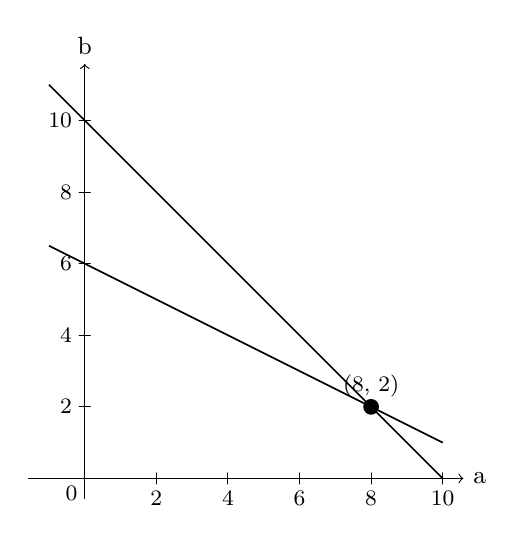
\begin{tikzpicture}
        \datavisualization [school book axes,
            visualize as smooth line/.list={a, b},
            visualize as scatter/.list={c},
            y axis={label=b, ticks={step=2}, length=5cm},
            x axis={label=a, ticks={step=2}, length=5cm}]

        data [format=function, set=a] {
                var x : interval [-1:10];
                func y = 10 - \value x;
            }
        data [format=function, set=b] {
                var x : interval [-1:10];
                func y =6 - \value x / 2;
            }
        info' {
        \fill [black] (visualization cs: x=8, y=2) circle [radius=1mm] node [above,font=\footnotesize] {(8, 2)};
        };
    \end{tikzpicture}
    \captionof{figure}{System 1}
\end{center}

\begin{center}
    \begin{tikzpicture}
        \datavisualization [school book axes,
            visualize as smooth line/.list={a, b},
            visualize as scatter/.list={c},
            y axis={label=b, ticks={step=2}, length=5cm},
            x axis={label=a, ticks={step=2}, length=5cm}]

        data [format=function, set=a] {
                var x : interval [-1:10];
                func y = 10 - \value x;
            }
        data [format=function, set=c] {
                var x : interval [-1:10];
                func y = 10 - \value x;
            };
    \end{tikzpicture}
    \captionof{figure}{System 2}
\end{center}

\begin{center}
    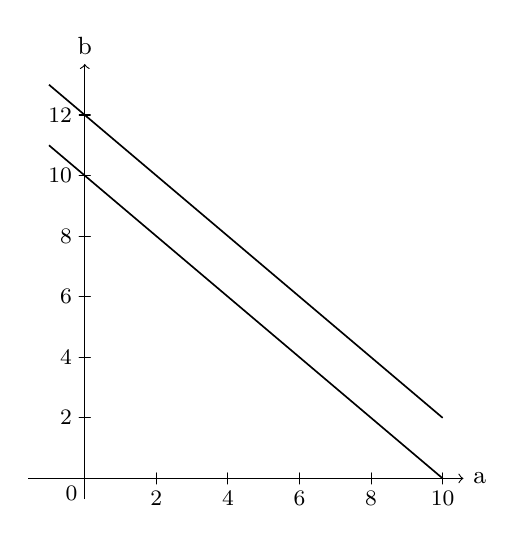
\begin{tikzpicture}
        \datavisualization [school book axes,
            visualize as smooth line/.list={a, b},
            visualize as scatter/.list={c},
            y axis={label=b, ticks={step=2}, length=5cm},
            x axis={label=a, ticks={step=2}, length=5cm}]

        data [format=function, set=a] {
                var x : interval [-1:10];
                func y = 10 - \value x;
            }
        data [format=function, set=b] {
                var x : interval [-1:10];
                func y = 12 - \value x;
            };
    \end{tikzpicture}
    \captionof{figure}{System 3}
\end{center}


\section{System of linear equations: 3 variables}

\end{document}